\documentclass{beamer}
\usepackage[francais]{babel}
\usepackage[T1]{fontenc}
\usepackage[utf8]{inputenc}
\usepackage{amsrefs}
\usepackage{graphicx}

\mode<presenation>
{ \usetheme{boxes} }

%\AtBeginSection[]{
%  \begin{frame}<beamer>
%  \frametitle{R\'esum\'e}
%  \tableofcontents[currentsection]
%  \end{frame}
%}

\title{Knot thickness computation in parallel}
\author{Mathias Carlen}
\date{11 june 2009}

\begin{document}

\frame{\titlepage}
\frame{\frametitle{Content}\tableofcontents}

%skeleton
%\section{Test}
%\frame{
%  \frametitle{1. titre}
%  \begin{itemize}
%  \item<2-> Bla 1
%  \item<3-> Bla bla 2
%  \end{itemize}
%}

\section{Curves and thickness}

\begin{frame}
\frametitle{Curves and thickness}

\begin{itemize}
 \item<1-> closed curve $\gamma(s)$, with $s$ arclength param.
 \item<2-> knot class
 \item<3-> maximal thick tube $\longrightarrow$ thickness $\Delta$.
\end{itemize}
\vspace{1cm}
\pause
\pause
\pause
\includegraphics[height=2cm]{global.pdf}\hspace{.2cm}
\pause
\includegraphics[height=2cm]{local.pdf}
\pause
\[
\Delta = min ( min_s r(s) , min_{dc} \frac{\gamma(s)-\gamma(t)}{2} )
\]
\end{frame}

\section{Motivation}
\begin{frame}
\frametitle{Motivation}
\begin{itemize}
\item<1-> Why parallelize?
\item<2-> Minimize $L[\gamma]/\Delta[\gamma]$
\item<3-> Monte carlo
\item<4-> Animation
\end{itemize}
\end{frame}

\section{Thickness Algorithm}

\begin{frame}
\frametitle{Thickness Algorithm}
\begin{itemize}
\item[(1)]<1-> Discretize $\gamma$ with biarcs
\item[(2)]<2-> Compute smallest local radius $r_i$
\item[(3)]<3-> Prepare a set of candidate arc pairs $(a_i,b_i)$
\item[(4)]<4-> Compute minimal distance between arcs
\item[(5)]<5-> Double criticality test
\item[(6)]<6-> Distance test
\item[(7)]<7-> Bisect remaining arc pairs ($1$ pair -> $4$ pairs)
\item[(8)]<8-> If not below some tolerance goto 4
\item[(9)]<9-> Return thickness
\end{itemize}
\end{frame}

\section{Parallelization}
%\subsection{Master/Slave work}
%\subsection{MPI}
%\subsection{Implementation details}
%\subsubsection{Custom datatypes}
%\subsubsection{Batching}

\begin{frame}
\frametitle{Parallelization (1)}
\includegraphics[height=.8\textheight]{parallel_algo_flowchart.pdf}
\end{frame}

\begin{frame}
\frametitle{Parallelization (2)}
\begin{itemize}
\item<1-> MPI
\item<2-> custom datatype \texttt{struct Candidate}
\item<3-> batching candidates
\end{itemize}
\end{frame}

\section{Experiments and benchmarks}
%\subsection{Hardware/Software used}
%\subsection{CPUs}
%\subsection{Knot data points}
%\subsection{Batching}
%\subsection{Knot shapes}
%\subsection{Master/slaves timing}

\begin{frame}
\frametitle{Experiments and benchmarks (1)}
Computed on cluster \texttt{lcvmlc2} using \texttt{mpich-mx}. \\
\vspace{.5cm}
\pause
Time vs. number of CPUs \\
\includegraphics[width=.75\textwidth]{time_vs_cpus.pdf}
\end{frame}

\begin{frame}
\frametitle{Experiments and benchmarks (2)}
Time vs. discretization \\
\includegraphics[width=.75\textwidth]{time_vs_nodes.pdf}
\end{frame}

\begin{frame}
\frametitle{Experiments and benchmarks (3)}
Time vs. batching \\
\includegraphics[width=.75\textwidth]{time_vs_batch.pdf}
\end{frame}

\begin{frame}
\frametitle{Experiments and benchmarks (4)}
Time vs. knot type \\
\includegraphics[width=.75\textwidth]{time_vs_knots.pdf}
\end{frame}

\begin{frame}
\frametitle{Experiments and benchmarks (5)}
Master/Slave timing \\[1cm]
\begin{tabular}{lclll}
knot & data points & master (sec) & slaves (sec) & total (sec) \\
j3.1 & 512 & 0.165336 & 2.092650 & 2.258000 \\
k3.1 & 160 & 0.016368 & 0.016206 & 0.032578 \\
k4.1 & 208 & 0.024819 & 0.018046 & 0.042868 \\
k5.1 & 232 & 0.031302 & 0.000165 & 0.031471 \\
k6.1 & 280 & 0.042829 & 0.000162 & 0.042995 \\
\end{tabular}
\end{frame}

\section{Possible improvements}
%\subsection{Master idle or not}
%\subsection{Master computes, interrupt system?}
%\subsection{Best value broadcast}
%\subsection{Optimize master initialization step}

\begin{frame}
\frametitle{Possible improvements}
\begin{itemize}
\item<1-> Master idle/working
\item<2-> Master computing (interrupt system)
\item<3-> Broadcast best current value
\item<4-> Optimize master init step
\end{itemize}
\end{frame}

\end{document}
